\documentclass[a4paper, 12pt]{article}

\usepackage[czech]{babel}
\usepackage[utf8]{inputenc}
\usepackage[total={17cm,25cm}, top=4cm, left=3cm, right=3cm, includefoot]{geometry}
\usepackage{graphicx}
\usepackage{subcaption}
\usepackage{caption}
\usepackage{mathtools}
\usepackage{xfrac}
\usepackage{enumerate}
\usepackage[hidelinks, unicode]{hyperref}
\usepackage{listings}
\usepackage{float}

\begin{document}

\begin{titlepage}

	\centering
	\begin{figure}
    \centering
	
\includegraphics[scale=2]{img/logo.pdf}\par\vspace{1cm}
	\end{figure}
	{\scshape\huge Západočeská Univerzita v Plzni \par}
	\vspace{0.5cm}
	{\scshape\LARGE Fakulta Aplikovaných Věd\par}
	\vspace{1.5cm}
	{\scshape\Large\ Operační systémy\par}
	\vspace{0.5cm}
	{\scshape\Large\ Semestrální práce \\ Simulace operačního systému DOS \par}
	\vspace{1cm}
	{\Large David Bohmann - A17N0064P\par}
	{\Large Jakub Váverka - A17N0095P\par}
	{\Large Václav Janoch - A17N0070P\par}
	\vfill
	{\large \today\par}
\end{titlepage}
\pagenumbering{gobble}
\tableofcontents

\newpage
\pagenumbering{arabic}
\section{Zadání}
\par Z nabízených možností jsme si vybrali zadání č. 3: Simulace operačního systému DOS.
\par Cílem práce bylo seznámení se s instrukční sadou pro procesory navazující na 16bitový procesor Intel 8086, pochopení toho jak probíhá klasický běh programů pod operačním systémem DOS a celkové seznámení s virtualizací.
\par K zadání byl přiložen jednak spustitelný soubor s koncovkou \textit{.com}, ale i zdrojový kód ze kterého byl vytvořen. Soubor \textit{VB08.COM} je spustitelný pod platformou MS-DOS. Abychom zjistili co přesně dělá, byli jsme nuceni tento soubor spustit v emulátoru DOSBox. Naším úkolem bylo tedy vytvoření takového programu, který by soubor načetl a provedl virtualizaci, abychom získali stejný výsledek, jako DOSBox.  
\subsection{Přesné znění zadání}
\begin{itemize}
\item Máte k dispozici malý program pro MS-DOS (com.zip)
\begin{itemize}
\item Včetně zdrojového kódu
\item A včetně kódu přeloženého do COM – tj. pouze sekvence, která se zavede do paměti a CS:IP se nastaví na první zavedený byte
\begin{itemize}
\item Před programem má být 100h bytů dlouhý Program Segment Prefix
\end{itemize}
\item Program si lze vyzkoušet např. v DOSBox
\end{itemize}
\item Implementujte minimální emulaci MS-DOSu, která vykoná tento program
\item Ve své podstatě je úloha o tom, jak se dělá emulace/paravirtualizace
\end{itemize}
\section{Zpracování}
Pro programování jsme se rozhodli použít programovací jazyk C, hlavně kvůli jednoduchému přistupování k paměti. Nejprve bylo nutné vytvořit struktury, které by dokázali simulovat strukturu architektury x86. 
\subsection{Registry}
Architektura x86 využívá pro své operace 8 aritmetických registrů, 4 segmentové, instrukční čítač a registr FLAGS. Důležité je si uvědomit, že mohou být operace volány nad různými částmi registrů. Je tedy nutné, abychom zařídili, že po přepsání spodní části registru se změní i hodnota celkového registru. Chtěl jsem tedy vytvořit několik ukazatelů do paměti, které budou ukazovat na ty samá čísla. Výsledek, ale vypadal dost nepřehledně. Naštěstí jsme narazili na takzvané uniony, které dělají v podstatě to samé a výsledný kód je mnohem přehlednější.
\subsubsection{Union}
Union má v programovacím jazyce C podobný zápis jako struktura. Jeho funkce je však úplně jiná. Místo toho, aby alokoval tolik paměti, kolik potřebuje na všechny své položky, alokuje jen velikost největší. Všechny jeho položky jsou poté umístěny na stejné místo v paměti. Přepsáním jedné, se přepíšou i ostatní. Tímto způsobem se tedy dají velice snadno nasimulovat registry. Na konzultacích jsme zjistili, že jsou takto vytvořené registry součástí zadání číslo 1. My jsme si ostatní zadání tak důkladně nepřečetli a tím pádem jsme si přidělali dost práce s vymýšlením naší struktury pro registry. 
\subsection{Paměť}
Nejprve jsme plánovali využít jen tolik paměti, kolik bude program skutečně potřebovat a alokovali jsme jen 500 bytů. V průběhu realizace jsme si však všimli, že program zapisuje přímo do video paměti, která je umístěna až na adrese 0xB800, proto jsme navýšili množství alokované paměti na 64 kB.
\subsection{Načtení souboru}
Po vytvoření struktur pro registry i paměť, jsme se mohli posunout k samotnému načtení do paměti. Z hlavičky souboru se zdrojovým kódem jsme zjistili, že se jedná o tiny režim a že načtený kód je posunutý o 100 bytů od začátku paměti. Načetli jsme tedy soubor \textit{VB08.COM} do paměti a nastavili instrukční čítač \textit{IP} na pozici první instrukce. Dále nás čekala nejtěžší část práce a to bylo pochopení toho, jak fungují opkódy.
\subsection{Opkódy}
\begin{figure}[H]
    \centering
	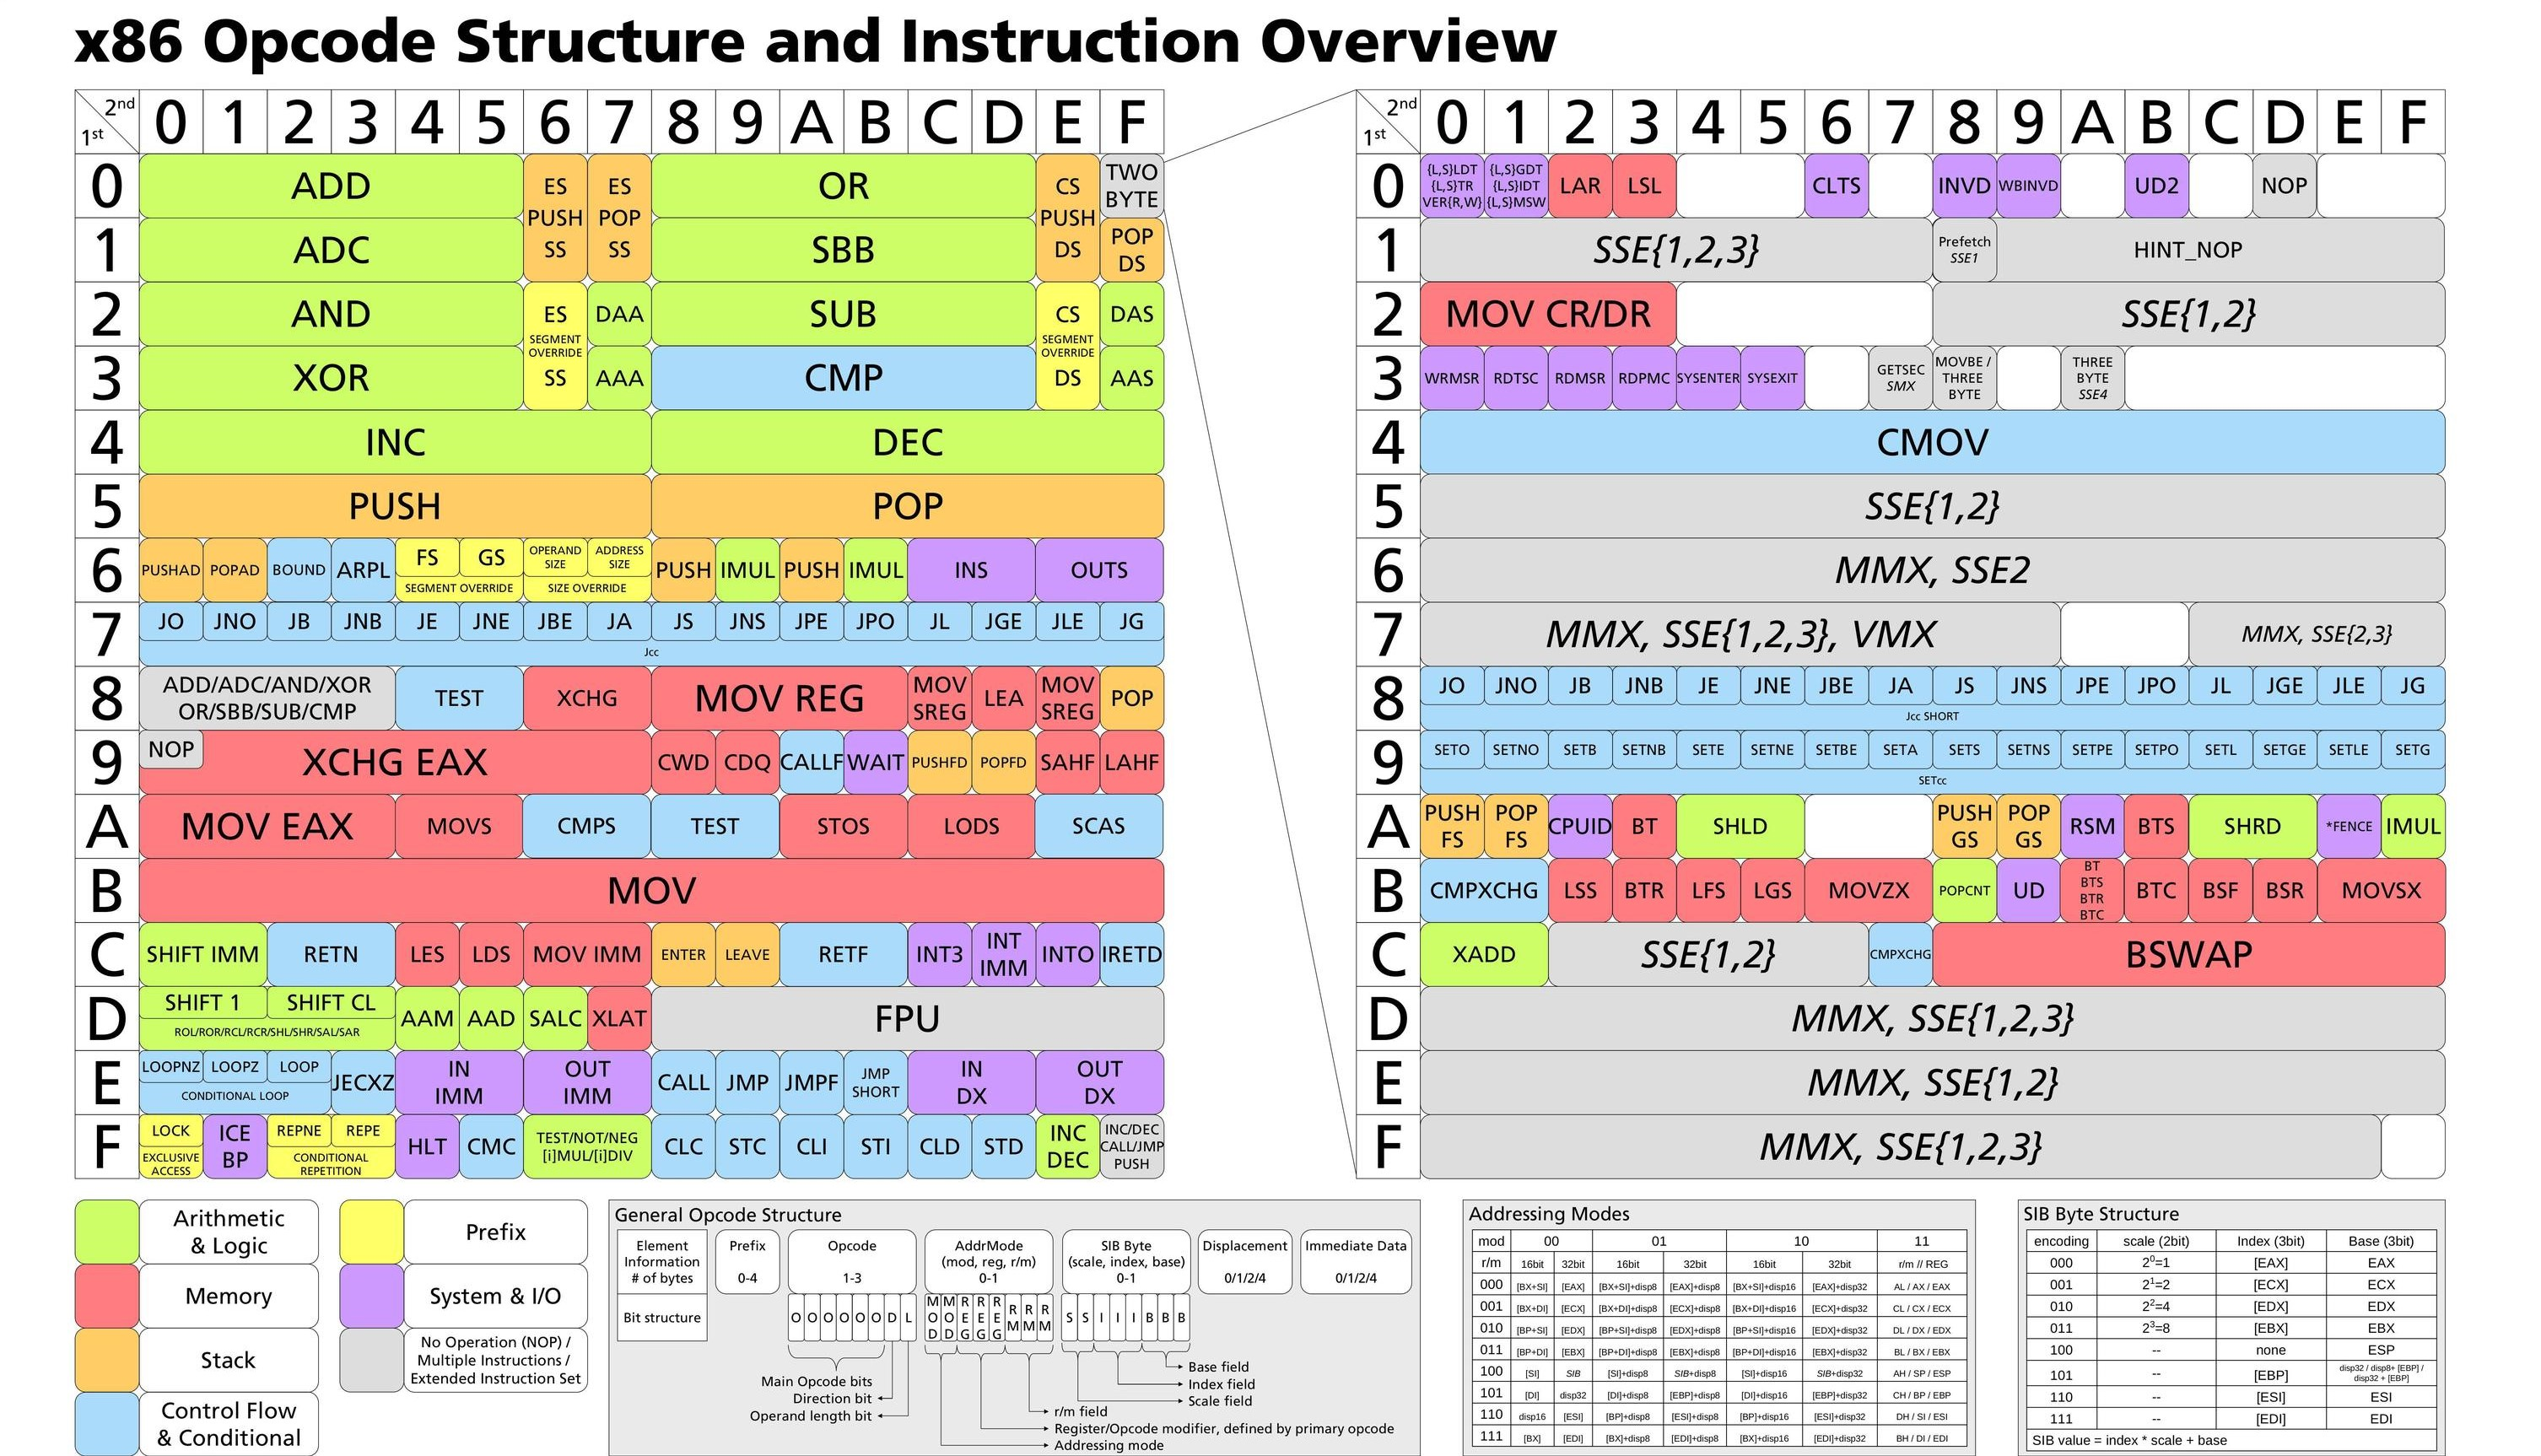
\includegraphics[width=\textwidth]{img/op.jpg}\par
    \caption{Tabulka opkódů}
  	\label{op}
\end{figure}
Z tabulky na obrázku \ref{op} lze snadno zjistit, jak se jmenují instrukce příslušící daným opkódům. Následovně bylo nutné nastudovat co přesně daná instrukce dělá a kolik k tomu využívá bytů. Je dobré si povšimnout, že například instrukce \textit{MOV} může být zapsána několika různými opkódy. Nejen \textit{MOV}, ale i ostatní instrukce mohou být dále modifikovány, jednak tímto způsobem, ale i následujícím bytem určujícím adresní mód, bytem SIB a nebo prefixem. Pochopení daných opkódů nebylo jednoduché, naštěstí jsme ale měli k dispozici zdrojový kód a tak jsme měli možnost zkontrolovat, zda se výsledná instrukce rovná té ze zdrojového kódu.
\subsection{Instrukce}
Rozhodli jsme se každou instrukci realizovat jako samostatnou funkci, která jako parametry dostane celkovou paměť a strukturu se všemi registry. Předtím, než jsme začali programovat samotnou logiku každé instrukce, jsme se je rozhodli pouze všechny načíst, abychom se ujistili, že odpovídají instrukcím ze souboru se zdrojovým kódem. Přišli jsme na to, že bude zapotřebí naprogramovat 22 instrukcí.
\begin{table}[h!]
\centering
\caption{Seznam implementovaných instrukcí}
\label{tab1}
\begin{tabular}{|l|l|}
\hline
Instrukce & Opkód \\\hline
add\_R8\_to\_RM8 & 0x00 \\
add & 0x03 \\
xor & 0x33 \\
increment\_EDX & 0x42 \\
increment\_EBX & 0x43 \\
decrement\_ECX & 0x49 \\
jump\_not\_equal & 0x75 \\
jump\_not\_parity & 0x7B \\
compare & 0x83 \\
move\_to\_R8 & 0x8A \\
move\_from\_segment & 0x8C \\
move\_to\_segment & 0x8E \\
move\_AH & 0xB4 \\
move\_AX & 0xB8 \\
move\_DX & 0xBA \\
move\_BX & 0xBB \\
move\_SI & 0xBE \\
move\_DI & 0xBF \\
move\_IMM16\_to\_RM16 & 0xC7 \\
interrupt & 0xCD \\
jump & 0xEB \\
increment & 0xFF \\\hline
\end{tabular}
\end{table}
Jako první instrukci jsme naprogramovali přerušení 20, který ukončí celý program. Díky tomu jsme mohli hned ze začátku udělat smyčku, která je ukončena až touto instrukcí. Uvnitř této smyčky byl zprvu vytvořený \textit{switch}, který rozhodoval, kterou funkci má spustit, podle přečteného opkódu. Po konzultacích jsme tento \textit{switch}, nakonec předělali na \textit{tabulku ukazatelů na funkce}. Kód je tedy tím pádem mnohem čitelnější a jednodušší na pochopení. Volání jednotlivých funkcí vypadá takto
\begin{lstlisting}[basicstyle=\small,language=C]
functions[(int) memory[dos_registers->ip]](memory, dos_registers);
\end{lstlisting}
\subsection{Prefixy}
Některé z instrukcí využívají prefixy. V našem programu se vykytují prefixy 3. Prefix 26, který značí \textit{Segment override}, 66 značí \textit{Operand override} a 67, který značí \textit{Address override}. Protože náš program načítá instrukce po bytech je nutné si prefix zapamatovat a použít ho při dalším cyklu. Rozhodli jsme se tedy do struktury s registry přidal \textit{flagy}, které ukládají stav prefixů předcházející samotné instrukci.
\subsection{Implementace instrukcí}
Samotná implementace jednotlivých instrukcí nebyla tak obtížná, jak jsme si zprvu mysleli. Těžké bylo převážně to, že jsme během implementace nevěděli, zda dané instrukce fungují přesně tak jak mají. Většinu instrukcí jsme však naprogramovali správně hned napoprvé a ty které fungovali chybně jsme dokázali snadno opravit s pomocí souboru se zdrojovým kódem.
\subsubsection{Skok -1}
Implementace skoku do sebe byla překvapivě jednoduchá. Po správné implementaci skoků a přeložení daného opkódu, jsme zjistili, že byt následující skok je opravdu číslo -1. Stačilo tedy přičíst výsledek k instrukčnímu čítači a instrukce proběhla přesně tak, jak měla.
\subsubsection{Přímý zápis do grafického bufferu}
Překvapil nás přímý zápis do grafického bufferu. Hlavně kvůli tomu, že jsme měli grafický buffer posunutý na jinou adresu. Po dokončení programu se tedy na obrazovku do pravého horního rohu nic nevypsalo. Naštěstí jsme po prozkoumání paměti řetězec našli a oprava byla jednoduchá.
\subsubsection{Přerušení}
Komplikovaná byla implementace přerušení. Naštěstí se v programu vyskytovali pouze 3. Ukončení programu a zápis do grafického bufferu byl ještě snadný, ale vypsání bufferu na obrazovku nám samotné zabralo několik hodin práce. Příjemné překvapení pro nás bylo, že i v současné konzoli operačního systému Windows 10, je možné vypsat barevně formátovaný výstup, jako tomu bylo u DOSu. 
\section{Dokumentace}
Kód je rozdělen do 5 souborů. Hlavní soubor \textit{main.c}. Tento soubor inicializuje registry a paměť, dále načte do paměti soubor \textit{VB08.COM} a začne provádět jednotlivé instrukce. Poté co přečte instrukci, která odpovídá přerušení 20, ukončí svůj běh a uvolní alokované struktury. Dále se v projektu nacházejí 2 hlavičkové soubory \textit{memory.h} a \textit{registers.h}. V souboru \textit{registers.h} je pomocí uninů definována hlavní struktura registrů. Tuto strukturu pak lze vypsat nebo inicializovat funkcemi ze souboru \textit{registers.c}. Druhý hlavičkový soubor se jmenuje \textit{memory.h} a obsahuje pomocné aliasy instrukcí a deklarace všech instrukčních funkcí. V souboru \textit{memory.c} je pak implementace jednotlivých instrukcí. Samotný běh programu probíhá podle diagramu na obrázku \ref{uml}.
\begin{table}[h!]
\centering
\caption{Soubory v projektu}
\label{tab2}
\begin{tabular}{|l|}
\hline
main.c\\
memory.c \\
memory.h \\
registers.c \\
registers.h \\\hline
\end{tabular}
\end{table}
\begin{figure}[H]
    \centering
	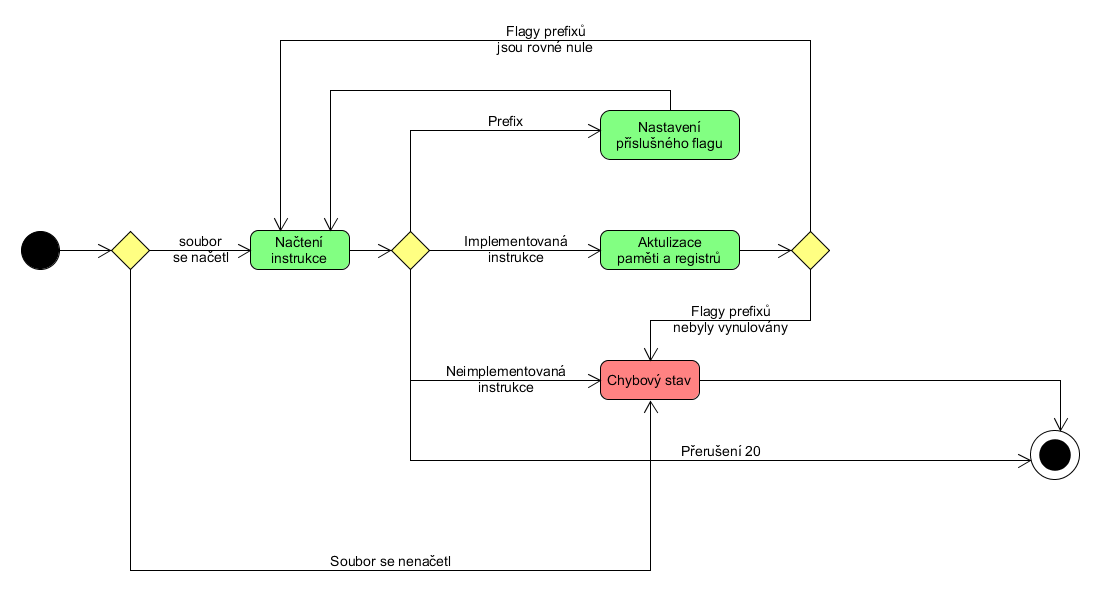
\includegraphics[width=\textwidth]{img/uml.png}\par
    \caption{Diagram běhu programu}
  	\label{uml}
\end{figure}
\section{Závěr}
Práce splňuje zadání v plném rozsahu. Obtížné bylo nastudování a pochopení toho co má vlastně být součástí práce, ale samotná implementace byla poměrně jednoduchá. Při této práci jsme se blízce seznámili s operačním systémem DOS, instrukční sadou x86 a tím jak probíhá emulace.
\end{document}